% Options for packages loaded elsewhere
\PassOptionsToPackage{unicode}{hyperref}
\PassOptionsToPackage{hyphens}{url}
\documentclass[
]{article}
\usepackage{xcolor}
\usepackage[margin=2.5cm]{geometry}
\usepackage{amsmath,amssymb}
\setcounter{secnumdepth}{-\maxdimen} % remove section numbering
\usepackage{iftex}
\ifPDFTeX
  \usepackage[T1]{fontenc}
  \usepackage[utf8]{inputenc}
  \usepackage{textcomp} % provide euro and other symbols
\else % if luatex or xetex
  \usepackage{unicode-math} % this also loads fontspec
  \defaultfontfeatures{Scale=MatchLowercase}
  \defaultfontfeatures[\rmfamily]{Ligatures=TeX,Scale=1}
\fi
\usepackage{lmodern}
\ifPDFTeX\else
  % xetex/luatex font selection
\fi
% Use upquote if available, for straight quotes in verbatim environments
\IfFileExists{upquote.sty}{\usepackage{upquote}}{}
\IfFileExists{microtype.sty}{% use microtype if available
  \usepackage[]{microtype}
  \UseMicrotypeSet[protrusion]{basicmath} % disable protrusion for tt fonts
}{}
\makeatletter
\@ifundefined{KOMAClassName}{% if non-KOMA class
  \IfFileExists{parskip.sty}{%
    \usepackage{parskip}
  }{% else
    \setlength{\parindent}{0pt}
    \setlength{\parskip}{6pt plus 2pt minus 1pt}}
}{% if KOMA class
  \KOMAoptions{parskip=half}}
\makeatother
\usepackage{longtable,booktabs,array}
\newcounter{none} % for unnumbered tables
\usepackage{calc} % for calculating minipage widths
% Correct order of tables after \paragraph or \subparagraph
\usepackage{etoolbox}
\makeatletter
\patchcmd\longtable{\par}{\if@noskipsec\mbox{}\fi\par}{}{}
\makeatother
% Allow footnotes in longtable head/foot
\IfFileExists{footnotehyper.sty}{\usepackage{footnotehyper}}{\usepackage{footnote}}
\makesavenoteenv{longtable}
\usepackage{graphicx}
\makeatletter
\newsavebox\pandoc@box
\newcommand*\pandocbounded[1]{% scales image to fit in text height/width
  \sbox\pandoc@box{#1}%
  \Gscale@div\@tempa{\textheight}{\dimexpr\ht\pandoc@box+\dp\pandoc@box\relax}%
  \Gscale@div\@tempb{\linewidth}{\wd\pandoc@box}%
  \ifdim\@tempb\p@<\@tempa\p@\let\@tempa\@tempb\fi% select the smaller of both
  \ifdim\@tempa\p@<\p@\scalebox{\@tempa}{\usebox\pandoc@box}%
  \else\usebox{\pandoc@box}%
  \fi%
}
% Set default figure placement to htbp
\def\fps@figure{htbp}
\makeatother
\setlength{\emergencystretch}{3em} % prevent overfull lines
\providecommand{\tightlist}{%
  \setlength{\itemsep}{0pt}\setlength{\parskip}{0pt}}
\usepackage{bookmark}
\IfFileExists{xurl.sty}{\usepackage{xurl}}{} % add URL line breaks if available
\urlstyle{same}
\hypersetup{
  hidelinks,
  pdfcreator={LaTeX via pandoc}}

\author{}
\date{}

\begin{document}

\section{A Thought Experiment on Double-Slit Interference from a
Localized Odd-Harmonic Source --- Shape Preservation Is Conditional and
Fragile, and the Single-Wavelength N=1 Is the Robust Special Case
(Alignment Condition, Tolerance Band, Off-axis
Scattering)}\label{a-thought-experiment-on-double-slit-interference-from-a-localized-odd-harmonic-source-shape-preservation-is-conditional-and-fragile-and-the-single-wavelength-n1-is-the-robust-special-case-alignment-condition-tolerance-band-off-axis-scattering}

\textbf{Noriaki Kihara}

\emph{This paper is a \textbf{thought experiment (model calculation)},
not a measurement. It contains no claim that overturns established
physics (standard wave optics / quantum mechanics). It illustrates and
organizes, by exact analysis and numerical computation, the far-field
interference when a \textbf{localized source} with positional
fluctuation is passed through a double slit. We take the preceding
position-readout paper {[}1{]} as the sole self-reference and limit
external citations to established textbook facts (spatial coherence /
far-field double slit; the closed form of the odd-harmonic cosine sum).}

Version v0.1 (2026-06-29) DOI (Version): 10.5281/zenodo.21035831 DOI
(Concept): 10.5281/zenodo.21035830 Zenodo:
https://zenodo.org/records/21035831

\begin{center}\rule{0.5\linewidth}{0.5pt}\end{center}

\subsection{Abstract}\label{abstract}

The preceding paper {[}1{]} showed that when a
\textbf{single-wavelength} point source has a positional fluctuation
\(P(y)\), in each trial the far-field double-slit fringe \textbf{shifts
by the pure geometric path difference while keeping its shape}, and that
over repeated trials the distribution of the fringe shift is the
push-forward of \(P\), which \textbf{preserves the shape} because the
map is linear in the paraxial regime (\(\cos^2\) if \(P=\cos^2\)).

This paper extends that to a \textbf{localized source wave}. We
represent the localization by a constant-amplitude odd-harmonic sum (the
isolated peak wave \(S_N\)) and pass it through the double slit. The
results are threefold.

\begin{enumerate}
\def\labelenumi{\arabic{enumi}.}
\tightlist
\item
  \textbf{Shape preservation (when aligned).} Although \(S_N\) is a sum
  of odd harmonics, it appears in the far field as a single, sharply
  localized fringe \textbf{without changing shape}. This holds only when
  the source--slit diagonal distance \(r_k=\sqrt{L^2+(W/2)^2}\) is
  ``aligned'' to an integer or half-integer multiple of the fundamental
  wavelength \(\lambda_0\):
  \[\sqrt{L^{2}+(W/2)^{2}}=\frac{m}{2}\,\lambda_0\qquad(m\in\mathbb{Z}).\]
\item
  \textbf{Sharp alignment condition.} Alignment is not a knife edge but
  a band of width \(\sim 1/(2N)\), narrowing as the highest odd-harmonic
  order \(N\) grows. A \textbf{slight difference} in \(\lambda_0\)
  (about \(3\%\) in our example) decides whether interference forms or
  scatters. The central-alignment tolerance band itself is
  \textbf{independent of \(W/L\)}; the effect of \(W\) appears as
  off-axis fragility (§3.3, §4.3).
\item
  \textbf{Inheritance and fragility of the \(\cos^2\) readout.} An
  aligned localized source still traces \(\cos^2\) in the fringe-shift
  distribution under positional fluctuation (inheriting the push-forward
  of {[}1{]}). But off-axis (\(y\neq0\)) the source--slit path
  difference becomes unequal on the two arms, the localization alignment
  breaks slightly, and the fringe peak shifts \textbf{downward} from
  \(\cos^2\). This departure grows with \(|y|\) and \(N\). The single
  wavelength (\(N=1\)) has none of this fragility and is
  \textbf{unconditional}; running our method at \(N=1\) under the same
  conditions reproduces {[}1{]} to machine precision (verified in §5).
\end{enumerate}

\textbf{The net new content of this paper is a negative result}:
localization (\(N\ge2\)) does not improve the simple push-forward of
{[}1{]}; it adds an \textbf{alignment constraint} (3.4) and
\textbf{off-axis fragility} that \(N=1\) did not have. Shape
preservation is real but \textbf{conditional and fragile}, and \(N=1\)
is the robust special case. For the broader program from localized waves
toward Born statistics, this fragility itself is an important finding.
These are not the derivation of a new probability law but illustrations
of the change of variables that maps the input distribution onto the
observed statistic (fringe shift), and of the alignment condition /
sensitivity / fragility of the interference of the odd-harmonic
localized wave. This paper is a thought experiment; it organizes
established physics rather than overturning it. We note that the
visibility loss from \textbf{intensity accumulation} of an extended
source (spatial coherence / van Cittert--Zernike theorem {[}2,3{]}) is a
different observation mode from the one of this paper (the push-forward
of the fringe shift) (§6.1).

\begin{center}\rule{0.5\linewidth}{0.5pt}\end{center}

\subsection{1. Introduction}\label{introduction}

Double-slit interference is a basic stage in wave optics and quantum
mechanics. The preceding paper {[}1{]} asked, for a \textbf{stationary
point source with positional fluctuation} (single wavelength
\(\lambda_0\)), what statistics appear in the fringe shift over repeated
observation, and showed: each trial shifts the same-shape fringe by the
geometric path difference; the shift is a nearly linear map of the
source position; hence drawing the source position repeatedly from
\(P(y)\), the fringe-shift distribution is the push-forward of \(P\),
preserving its shape in the paraxial regime.

Here we replace the source of that setting by a \textbf{localized wave}.
That is, instead of the single-wavelength \(\cos\) of a point source, we
take as the source waveform a wave \(S_N\) that is sharply localized at
the center by superposing constant-amplitude odd harmonics. We ask two
things: (i) does the localized wave, which is a sum of odd harmonics,
localize in the far field \textbf{while preserving its shape}, and under
what conditions; (ii) when that localized source has positional
fluctuation, is the \(\cos^2\) readout of {[}1{]} \textbf{inherited, or
does it break down}.

We take the same geometry as {[}1{]} (\(L=10\), \(W=5\), \(\lambda_0\)
the fundamental wavelength). Everything is an exact computation on the
specified configuration; this is a thought experiment. The notation and
the closed form of the cosine sum follow a standard analysis text
{[}4{]}; the far-field double slit and spatial coherence follow standard
optics texts {[}2,3{]}.

\begin{center}\rule{0.5\linewidth}{0.5pt}\end{center}

\subsection{2. The localized odd-harmonic
source}\label{the-localized-odd-harmonic-source}

\subsubsection{\texorpdfstring{2.1 The isolated peak wave
\(S_N\)}{2.1 The isolated peak wave S\_N}}\label{the-isolated-peak-wave-s_n}

On the half-wave phase interval \(\varphi\in[-\pi/2,\pi/2]\), define the
constant-amplitude odd-harmonic cosine sum

\[
S_N(\varphi)=\sum_{m=0}^{(N-1)/2}\cos\!\big((2m+1)\varphi\big)
=\frac{\sin\!\big((N+1)\varphi\big)}{2\sin\varphi}
\tag{2.1}
\]

(\(N\) the highest odd-harmonic order, odd; the right-hand side is the
closed form of the cosine sum of an arithmetic progression {[}4{]}).
\(S_N\) has a central peak \(S_N(0)=(N+1)/2\) at \(\varphi=0\) and is
zero at the ends \(\varphi=\pm\pi/2\) --- an ``isolated peak wave.'' For
the observable we use the non-negative squared amplitude \(|S_N|^2\),
whose central peak width narrows as \(1/(N+1)\) (Fig 1).

\begin{figure}
\centering
\pandocbounded{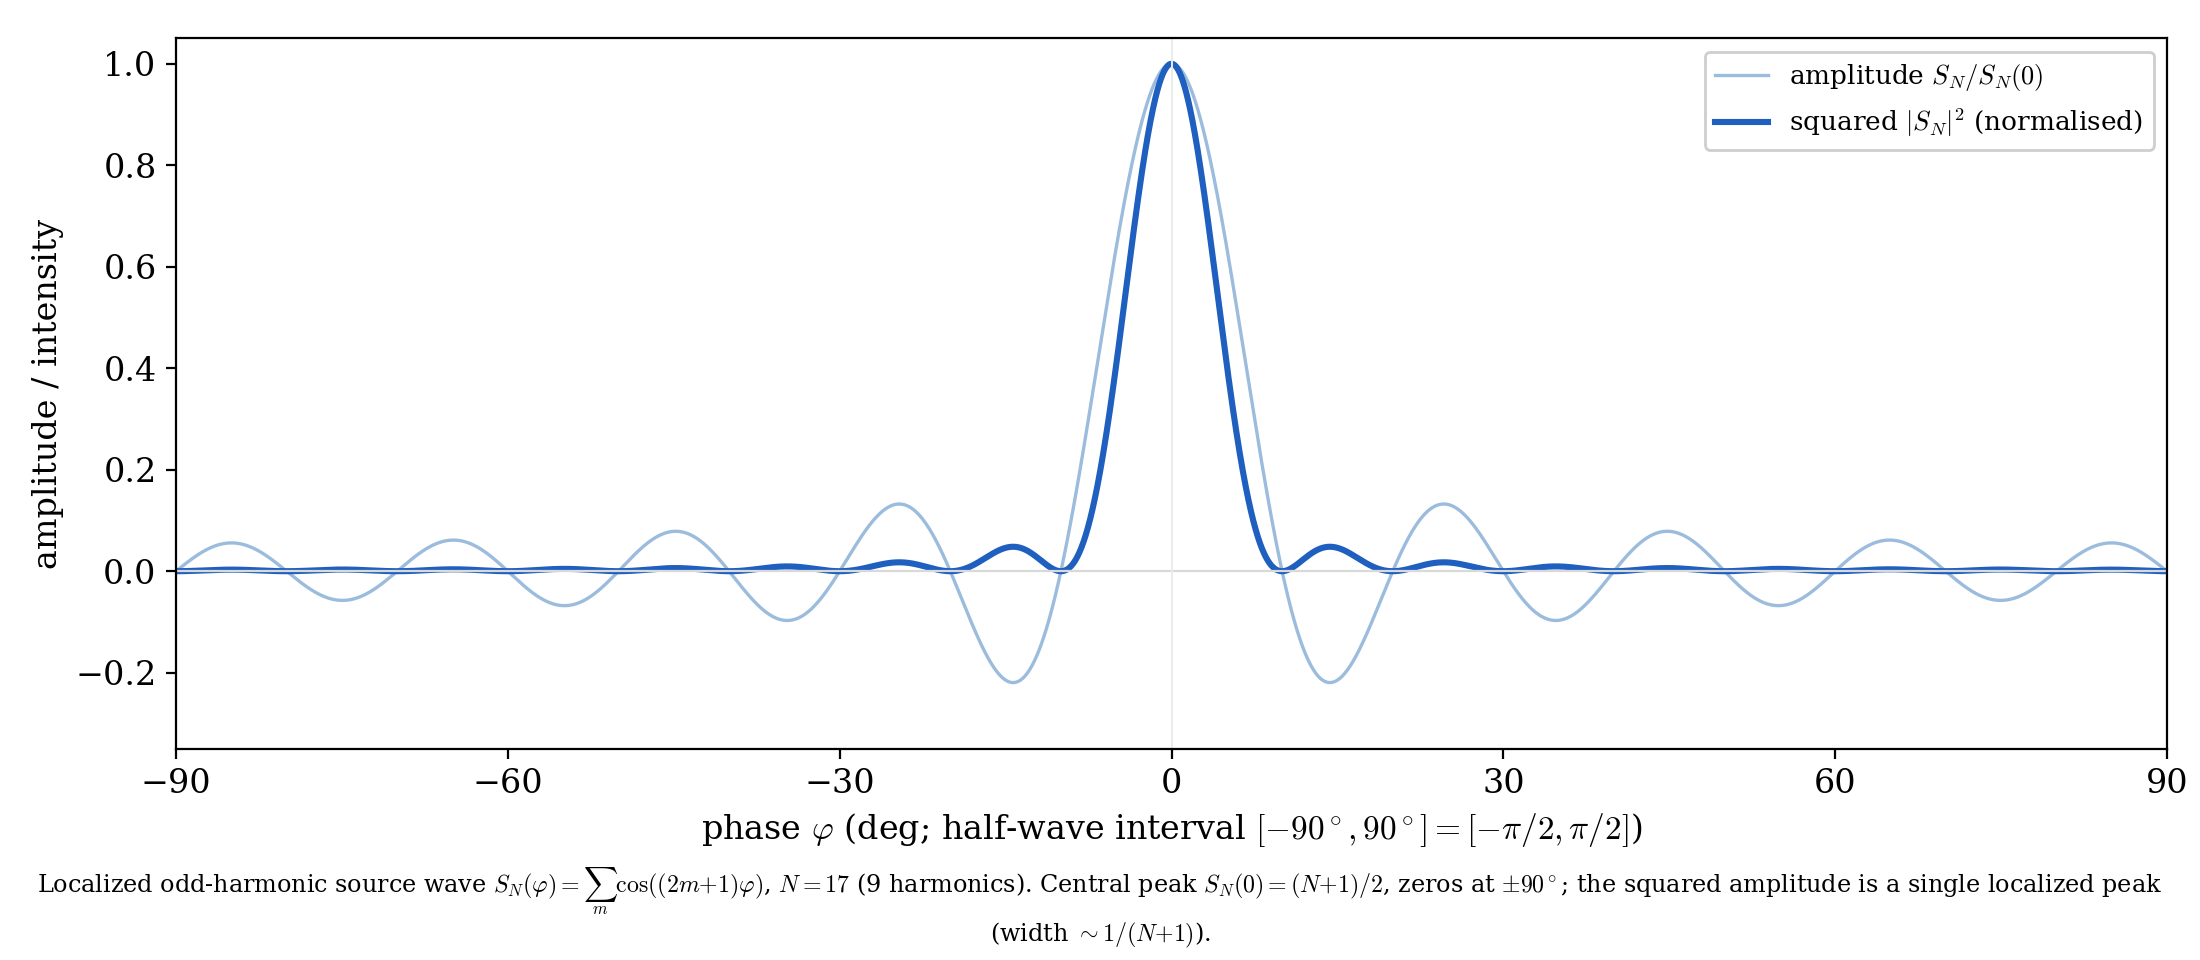
\includegraphics[keepaspectratio,alt={Fig 1 localized odd-harmonic source wave S\_N (N=17)}]{fig_paper2_localized_wave_N17.png}}
\caption{Fig 1 localized odd-harmonic source wave S\_N (N=17)}
\end{figure}

\emph{Fig 1: The localized source wave
\(S_N(\varphi)=\sum_m\cos((2m+1)\varphi)\) (\(N=17\), 9 odd harmonics).
Thin line: normalized amplitude \(S_N/S_N(0)\); thick line: normalized
squared amplitude \(|S_N|^2\). A single sharp localized peak at the
center, zero at the ends \(\pm90^\circ\). The fundamental frequency
\(\nu=1\) and wavelength \(\lambda_0\) are unchanged by the harmonic
carving (\(\gcd(1,3,\dots,N)=1\)).}

\subsubsection{\texorpdfstring{2.2 The fundamental wavelength
\(\lambda_0\) (cage) and the
harmonics}{2.2 The fundamental wavelength \textbackslash lambda\_0 (cage) and the harmonics}}\label{the-fundamental-wavelength-lambda_0-cage-and-the-harmonics}

We call the fundamental wavelength \(\lambda_0\) (the longest wavelength
= the \(n=1\) wavelength) the ``cage.'' The harmonic wavelengths are
\(\lambda_n=\lambda_0/n\) (\(n=1,3,\dots,N\)), and \(\lambda_0\) gives
the spatial period of the localized wave. \(\nu=1,\lambda_0\) is a
relative normalization; the odd harmonics only change the sharpness of
the localization (relative width \(1/(N+1)\)) and do not change the
fundamental frequency / wavelength.

\begin{center}\rule{0.5\linewidth}{0.5pt}\end{center}

\subsection{3. Alignment condition and shape
preservation}\label{alignment-condition-and-shape-preservation}

\subsubsection{3.1 Far-field double slit
(exact)}\label{far-field-double-slit-exact}

Let the source be \(S=(-L,\,y)\) and the slits \(A_1=(0,+W/2)\),
\(A_2=(0,-W/2)\). The screen point is parametrized by the far-field
diffraction angle \(\theta_s\) (\(s=\sin\theta_s\)). The wavelength is
each \(\lambda_n\) everywhere (no motion assumption, no Doppler). The
phase of each harmonic \(n\) and arm \(k\) is the sum of the source-side
geometric path and the far-field screen-side path difference:

\[
\Phi_k^{(n)}(s;y)=\frac{2\pi n}{\lambda_0}\Big[\,r_k(y)-y_{{\rm slit},k}\,s\,\Big],
\qquad r_k(y)=\sqrt{L^2+(y-y_{{\rm slit},k})^2}
\tag{3.1}
\]

(the harmonic version of the formula in {[}1{]};
\(2\pi/\lambda_n=2\pi n/\lambda_0\)). The total complex amplitude and
intensity (exact Born form via complex conjugation) are

\[
\psi(s;y)=\sum_{n}\Big[e^{i\Phi_1^{(n)}}+e^{i\Phi_2^{(n)}}\Big],
\qquad I(s;y)=\big|\psi(s;y)\big|^2.
\tag{3.2}
\]

\subsubsection{\texorpdfstring{3.2 The alignment condition for the
centered source
\(y=0\)}{3.2 The alignment condition for the centered source y=0}}\label{the-alignment-condition-for-the-centered-source-y0}

For the centered source, \(r_1=r_2=r_k\equiv\sqrt{L^2+(W/2)^2}\), and
(3.2) becomes

\[
\psi(s;0)=\sum_n e^{\,i(2\pi n/\lambda_0)\,r_k}\cdot 2\cos\!\Big(\frac{2\pi n}{\lambda_0}\frac{W}{2}\,s\Big).
\tag{3.3}
\]

\textbf{The source-side phase \(e^{i(2\pi n/\lambda_0)r_k}\) is common
to both slits but differs per harmonic \(n\).} The condition that it
align over all odd \(n\) (factor out as a common factor) is that
\(2\pi n\,r_k/\lambda_0\) be the same value (mod \(2\pi\)) independent
of \(n\), i.e.

\[
\boxed{\ \frac{r_k}{\lambda_0}=\frac{m}{2}\ \ (m\in\mathbb{Z}),\quad\text{i.e.}\quad
\sqrt{L^{2}+(W/2)^{2}}=\frac{m}{2}\,\lambda_0\ }
\tag{3.4}
\]

(\(m\) even gives phase \(+1\), \(m\) odd gives \((-1)^n=-1\); both
align identically after squaring). Physically it means ``the
source--slit diagonal distance is an integer/half-integer number of
fundamental wavelengths, i.e.~the slit sits on a spike (node) of the
localized wave.''

When aligned, (3.3) becomes
\(\psi(s;0)=({\rm common\ factor})\cdot 2\,S_N(\theta)\),
\(I=4\,S_N(\theta)^2\) (\(\theta=\pi W s/\lambda_0\)), so \textbf{the
screen interference intensity is the square of the localized wave
itself}. Since \(|S_N|^2\) has period \(180^\circ\) in \(\theta\), this
is strictly \textbf{the central one of a periodic train of fringes} (the
physical screen \(|s|\le1\) can carry several per side), whose center
appears, although a sum of odd harmonics, as a single sharply localized
fringe \textbf{without shape change} (Fig 2). Note that \(4S_N^2\) is
the \textbf{instantaneous coherent image} of
\(\omega,3\omega,5\omega,\dots\) phase-locked (a frequency comb),
including inter-harmonic cross terms. Under time-averaging by a slow
detector the cross terms drop and it reverts to a sum of single-harmonic
fringes; this paper treats the instantaneous image as a phase-domain
thought experiment.

\begin{figure}
\centering
\pandocbounded{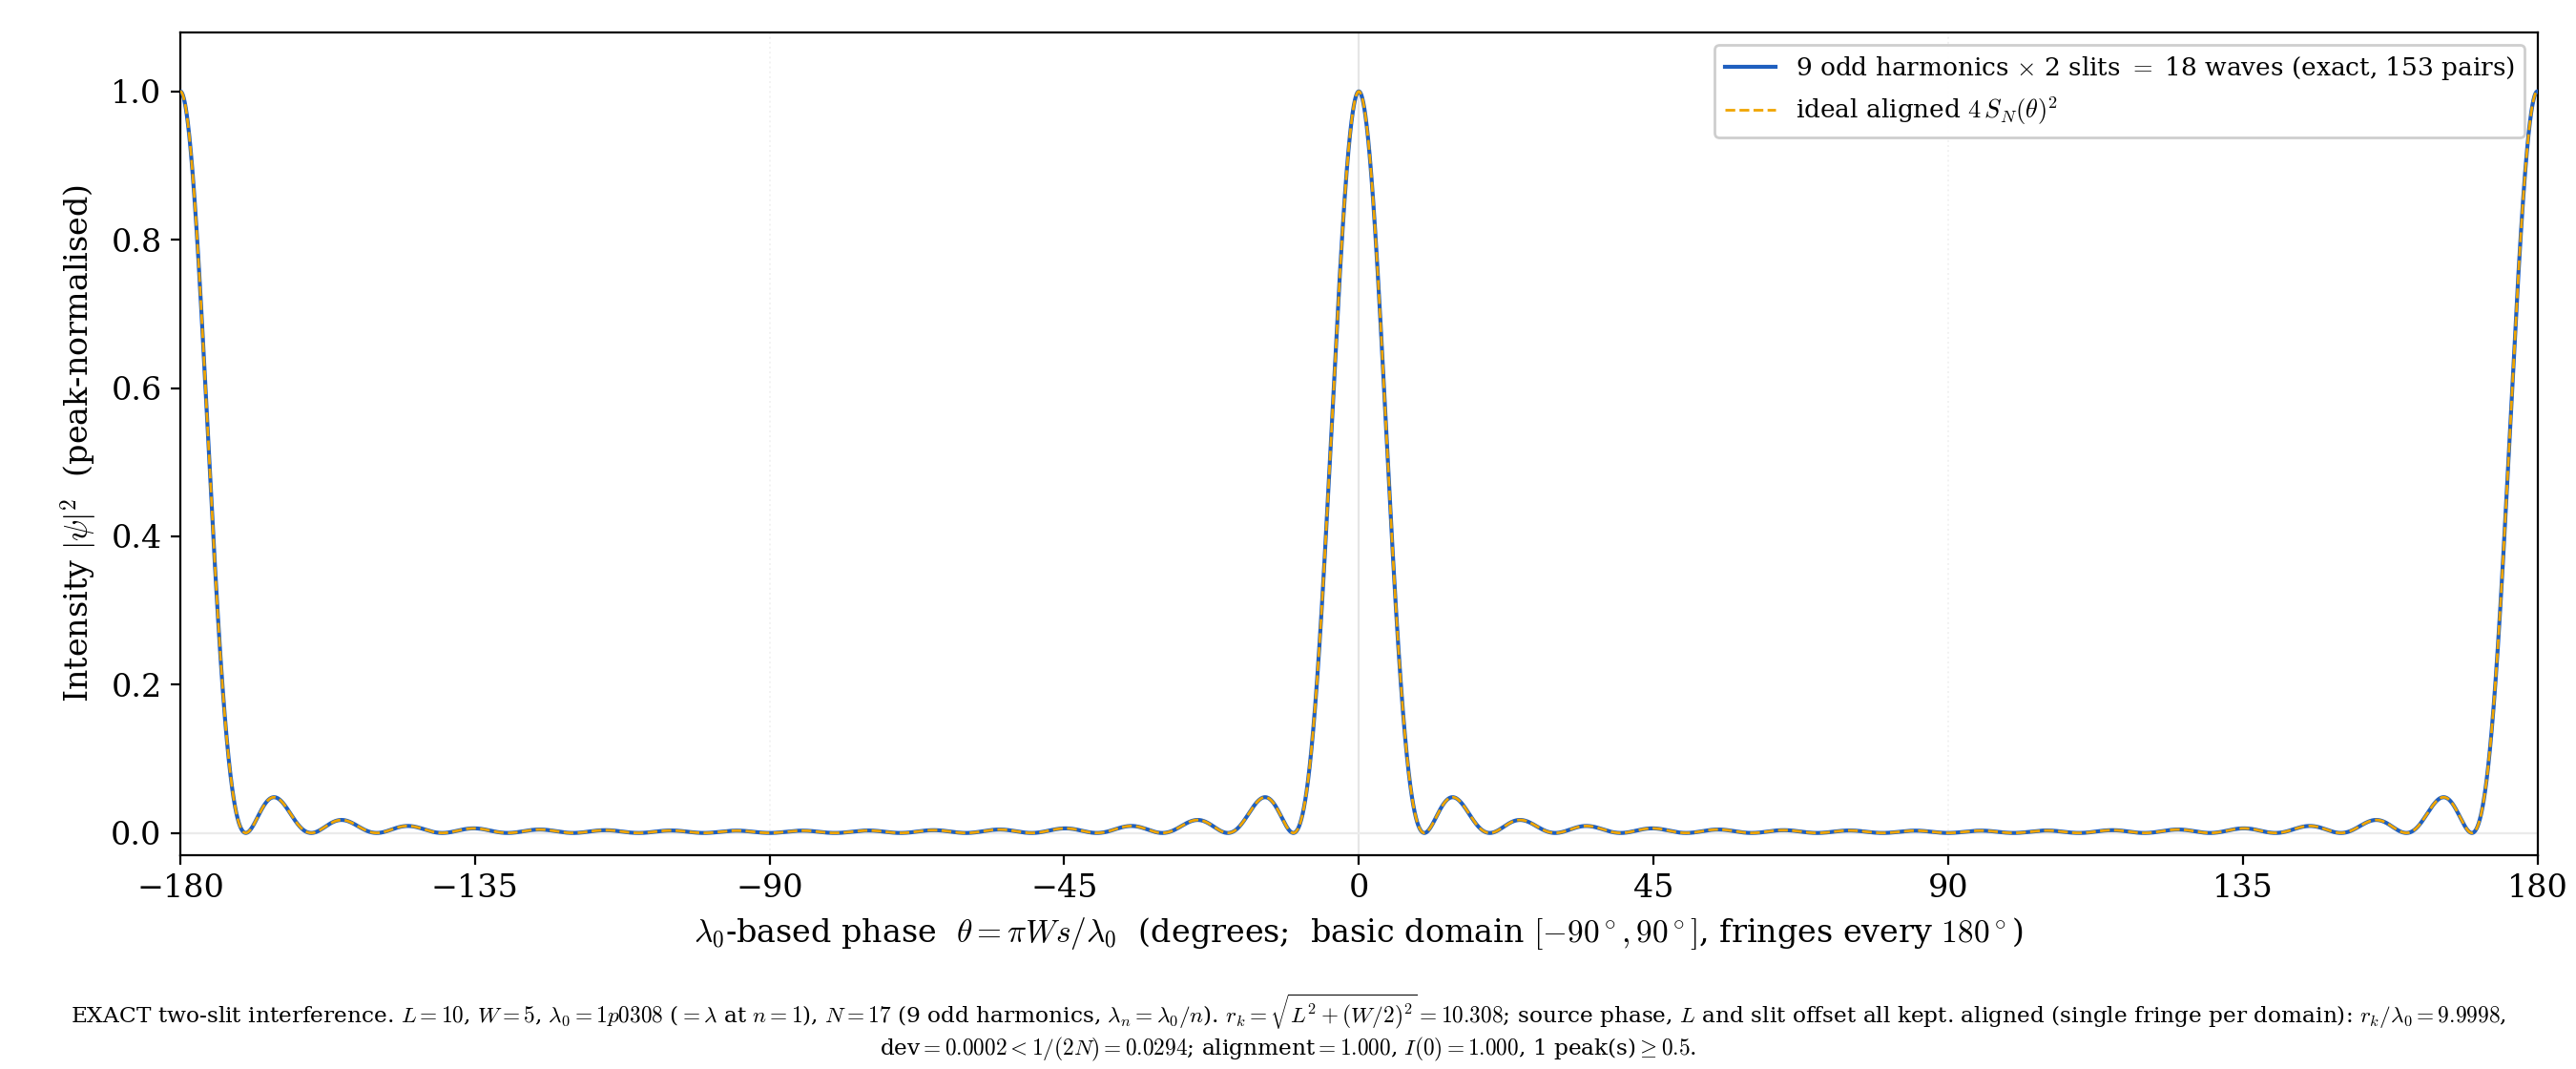
\includegraphics[keepaspectratio,alt={Fig 2 aligned shape-preserving interference (L=10, W=5, λ0=1.0308, N=17)}]{fig_oddharm_interference_L10_W5_lam1p0308_N17_pm180.png}}
\caption{Fig 2 aligned shape-preserving interference (L=10, W=5,
λ0=1.0308, N=17)}
\end{figure}

\emph{Fig 2: Far-field intensity of the aligned centered source
(\(y=0\)) (\(L=10\), \(W=5\), \(\lambda_0=1.0308\), \(N=17\),
\(r_k/\lambda_0=10.000\)). 18 waves (9 odd harmonics × 2 slits) are
summed exactly and squared. A single sharply localized fringe at the
center (the central one of a period-\(180^\circ\) train; several lie
within \(|s|\le1\)), \(I(0)=1\). Dashed: theory \(4S_N(\theta)^2\),
machine-precision agreement. Horizontal axis: \(\lambda_0\)-based phase
\(\theta=\pi W s/\lambda_0\).}

\subsubsection{\texorpdfstring{3.3 Sensitivity: the tolerance band
\(\sim 1/(2N)\) and where the \(W\)-dependence
lives}{3.3 Sensitivity: the tolerance band \textbackslash sim 1/(2N) and where the W-dependence lives}}\label{sensitivity-the-tolerance-band-sim-12n-and-where-the-w-dependence-lives}

Alignment is a band, not a knife edge. The phase error grows as
\(2\pi N\cdot\delta(r_k/\lambda_0)\) at the highest harmonic, so the
tolerance is

\[
\big|\,r_k/\lambda_0-\tfrac{m}{2}\,\big|\ \lesssim\ \frac{1}{2N},
\tag{3.5}
\]

narrower as \(N\) grows. For our geometry (\(L=10\), \(W=5\)),
\(r_k=\sqrt{106.25}=10.3078\). With \(\lambda_0=1\),
\(r_k/\lambda_0=10.308\), whose distance from the nearest half-integer
\(10.5\) is \(0.192\). This fits the band (3.5) only for
\(N<1/(2\cdot0.192)\approx2.6\), i.e.~\textbf{only \(N=1\) among odd
\(N\)}. By contrast \(\lambda_0=1.0308\) (\(r_k/\lambda_0=10.000\), a
mere \(\approx3\%\) change of \(\lambda_0\)) aligns comfortably even at
\(N=17\) (tolerance \(\pm0.029\)). \textbf{A slight difference in
\(\lambda_0\) decides interference vs scattering.}

The required wavelength-matching relative precision is of order
\(\sim 1/(2N\cdot r_k/\lambda_0)\) (\(r_k/\lambda_0\approx10\), so about
\(0.3\%\) at \(N=17\), \(0.05\%\) at \(N=99\)). Note that scaling the
whole geometry while keeping the ratio \(W/L\) fixed leaves
\(r_k/\lambda_0\) unchanged, so a bad ratio cannot be fixed by scaling
(\(r_k/L=\sqrt{1+(W/2L)^2}\) is generally irrational, but this holds
regardless of how large \(W/L\) is). To satisfy alignment, tune the two
free parameters \(L\) and \(\lambda_0\) to (3.4). \textbf{The
central-alignment tolerance band (3.5) is itself independent of \(W/L\),
equal to \(\sim1/(2N)\)}; the effect of \(W\) appears not in central
alignment but as \textbf{off-axis fragility (when the source leaves the
center)} (quantified in §4.3).

\begin{center}\rule{0.5\linewidth}{0.5pt}\end{center}

\subsection{\texorpdfstring{4. The \(\cos^2\) readout under positional
fluctuation}{4. The \textbackslash cos\^{}2 readout under positional fluctuation}}\label{the-cos2-readout-under-positional-fluctuation}

\subsubsection{4.1 The fluctuation setting (identical to
{[}1{]})}\label{the-fluctuation-setting-identical-to-1}

We assign the source position \(y\) a fluctuation and take, as in
{[}1{]}, the transverse-position probability distribution

\[
P(y)=\cos^2\!\Big(\frac{\pi y}{\Delta\lambda}\Big),\qquad y\in\Big[-\frac{\Delta\lambda}{2},\,\frac{\Delta\lambda}{2}\Big]
\tag{4.1}
\]

(central peak, zero at the ends; full width \(\Delta\lambda\),
half-range \(\Delta\lambda/2\); \(\Delta\lambda=\lambda_0\) corresponds
to the \(\pm\lambda/2\) of {[}1{]}). The source position is quasi-static
within a trial and re-drawn between trials according to \(P(y)\). The
experiments so far (§3, no fluctuation) correspond to
\(\Delta\lambda=0\).

\begin{figure}
\centering
\pandocbounded{\includegraphics[keepaspectratio,alt={Fig 3 source with positional fluctuation (the setup of {[}1{]})}]{fig_setup_source_uncertainty.png}}
\caption{Fig 3 source with positional fluctuation (the setup of
{[}1{]})}
\end{figure}

\emph{Fig 3: Magnified view of the source--slit region (from {[}1{]},
\(L=10\), \(W=5\)). The source position has an uncertainty of radius
\(\sim\lambda/2\), and along the axis parallel to the screen rides the
distribution \(P(y)=\cos^2\) (central peak, zero at the ends). This
paper replaces this source by the localized wave \(S_N\).}

\subsubsection{4.2 Push-forward of the fringe shift (exact
computation)}\label{push-forward-of-the-fringe-shift-exact-computation}

For each source position \(y\) we compute (3.2) exactly (off-axis
\(r_1(y)\neq r_2(y)\), keeping all source-side phases), weight by
\(P(y)\), and normalize by the central peak at \(y=0\). The central peak
of the localized fringe stands where the difference phases of all
harmonics align, \(\Delta r(y)-Ws=0\), at the position

\[
\Delta r(y)=r_1(y)-r_2(y)\ \approx\ -\frac{W}{L}\,y\ (\text{length, linear in the paraxial regime}),
\qquad
u(y)=\frac{2\pi}{\lambda_0}\,\Delta r(y)\ \approx\ -\frac{2\pi W}{L\lambda_0}\,y\ (\text{phase})
\tag{4.2}
\]

which is identical to the single-wavelength fringe shift of {[}1{]}.
Hence the fringe-shift distribution is the push-forward
\(\rho(u)=P(y(u))|dy/du|\) of \(P\), preserving the \(\cos^2\) shape in
the paraxial regime.

\subsubsection{4.3 Results: inheritance, fragility, and
scattering}\label{results-inheritance-fragility-and-scattering}

\textbf{(a) \(N=1\) (single wavelength, reproducing {[}1{]}).} With only
one harmonic, the source-side phase \(e^{i\kappa_1 r_k}\) is a mere
overall phase and cancels in \(|\psi|^2\). Hence the alignment condition
(3.4) is \textbf{not needed}: whatever \(L,W,\lambda_0\), the fringe
shifts in shape and the peaks trace \(\cos^2\). Running our method at
\(N=1\) under the same conditions (\(L=10\), \(W=5\), \(\lambda_0=1\),
\(\Delta\lambda=1\)) agrees with {[}1{]}'s figure
(fig\_decomposition\_static) in \textbf{all numbers and the whole curve
to machine precision (\(\le 2\times10^{-16}\))} (§5).

\begin{figure}
\centering
\pandocbounded{\includegraphics[keepaspectratio,alt={Fig 4 N=1 positional-fluctuation readout (machine-precision match with {[}1{]})}]{fig_oddharm_fluct_L10_W5_lam1_N1_dlam1.png}}
\caption{Fig 4 N=1 positional-fluctuation readout (machine-precision
match with {[}1{]})}
\end{figure}

\emph{Fig 4: \(N=1\), \(L=10\), \(W=5\), \(\lambda_0=1\),
\(\Delta\lambda=1\). The exact two-slit intensity of each source
\(y=x\,\Delta\lambda/2\) (\(x\in[-0.8,0.8]\)) is weighted by
\(P(y)=\cos^2(\pi x/2)\) and normalized by the \(y=0\) peak. The fringe
peaks (red) trace the \(\cos^2\) push-forward (yellow). This is exactly
{[}1{]}, and serves as the verification that the base of this paper
agrees with {[}1{]}.}

\textbf{(b) \(N=17\), misaligned (\(\lambda_0=1\)).} As in §3.3, with
\(\lambda_0=1\), \(N=17\) is outside the tolerance band, and \textbf{the
localization fails already at \(y=0\)} (central coherence
\(\approx25\%\)). The fringe splits into multiple peaks and the peaks
depart greatly from \(\cos^2\) (Fig 5). This is not a fluctuation
effect; it shows that \textbf{a misaligned localized source does not
interfere/localize at all.}

\begin{figure}
\centering
\pandocbounded{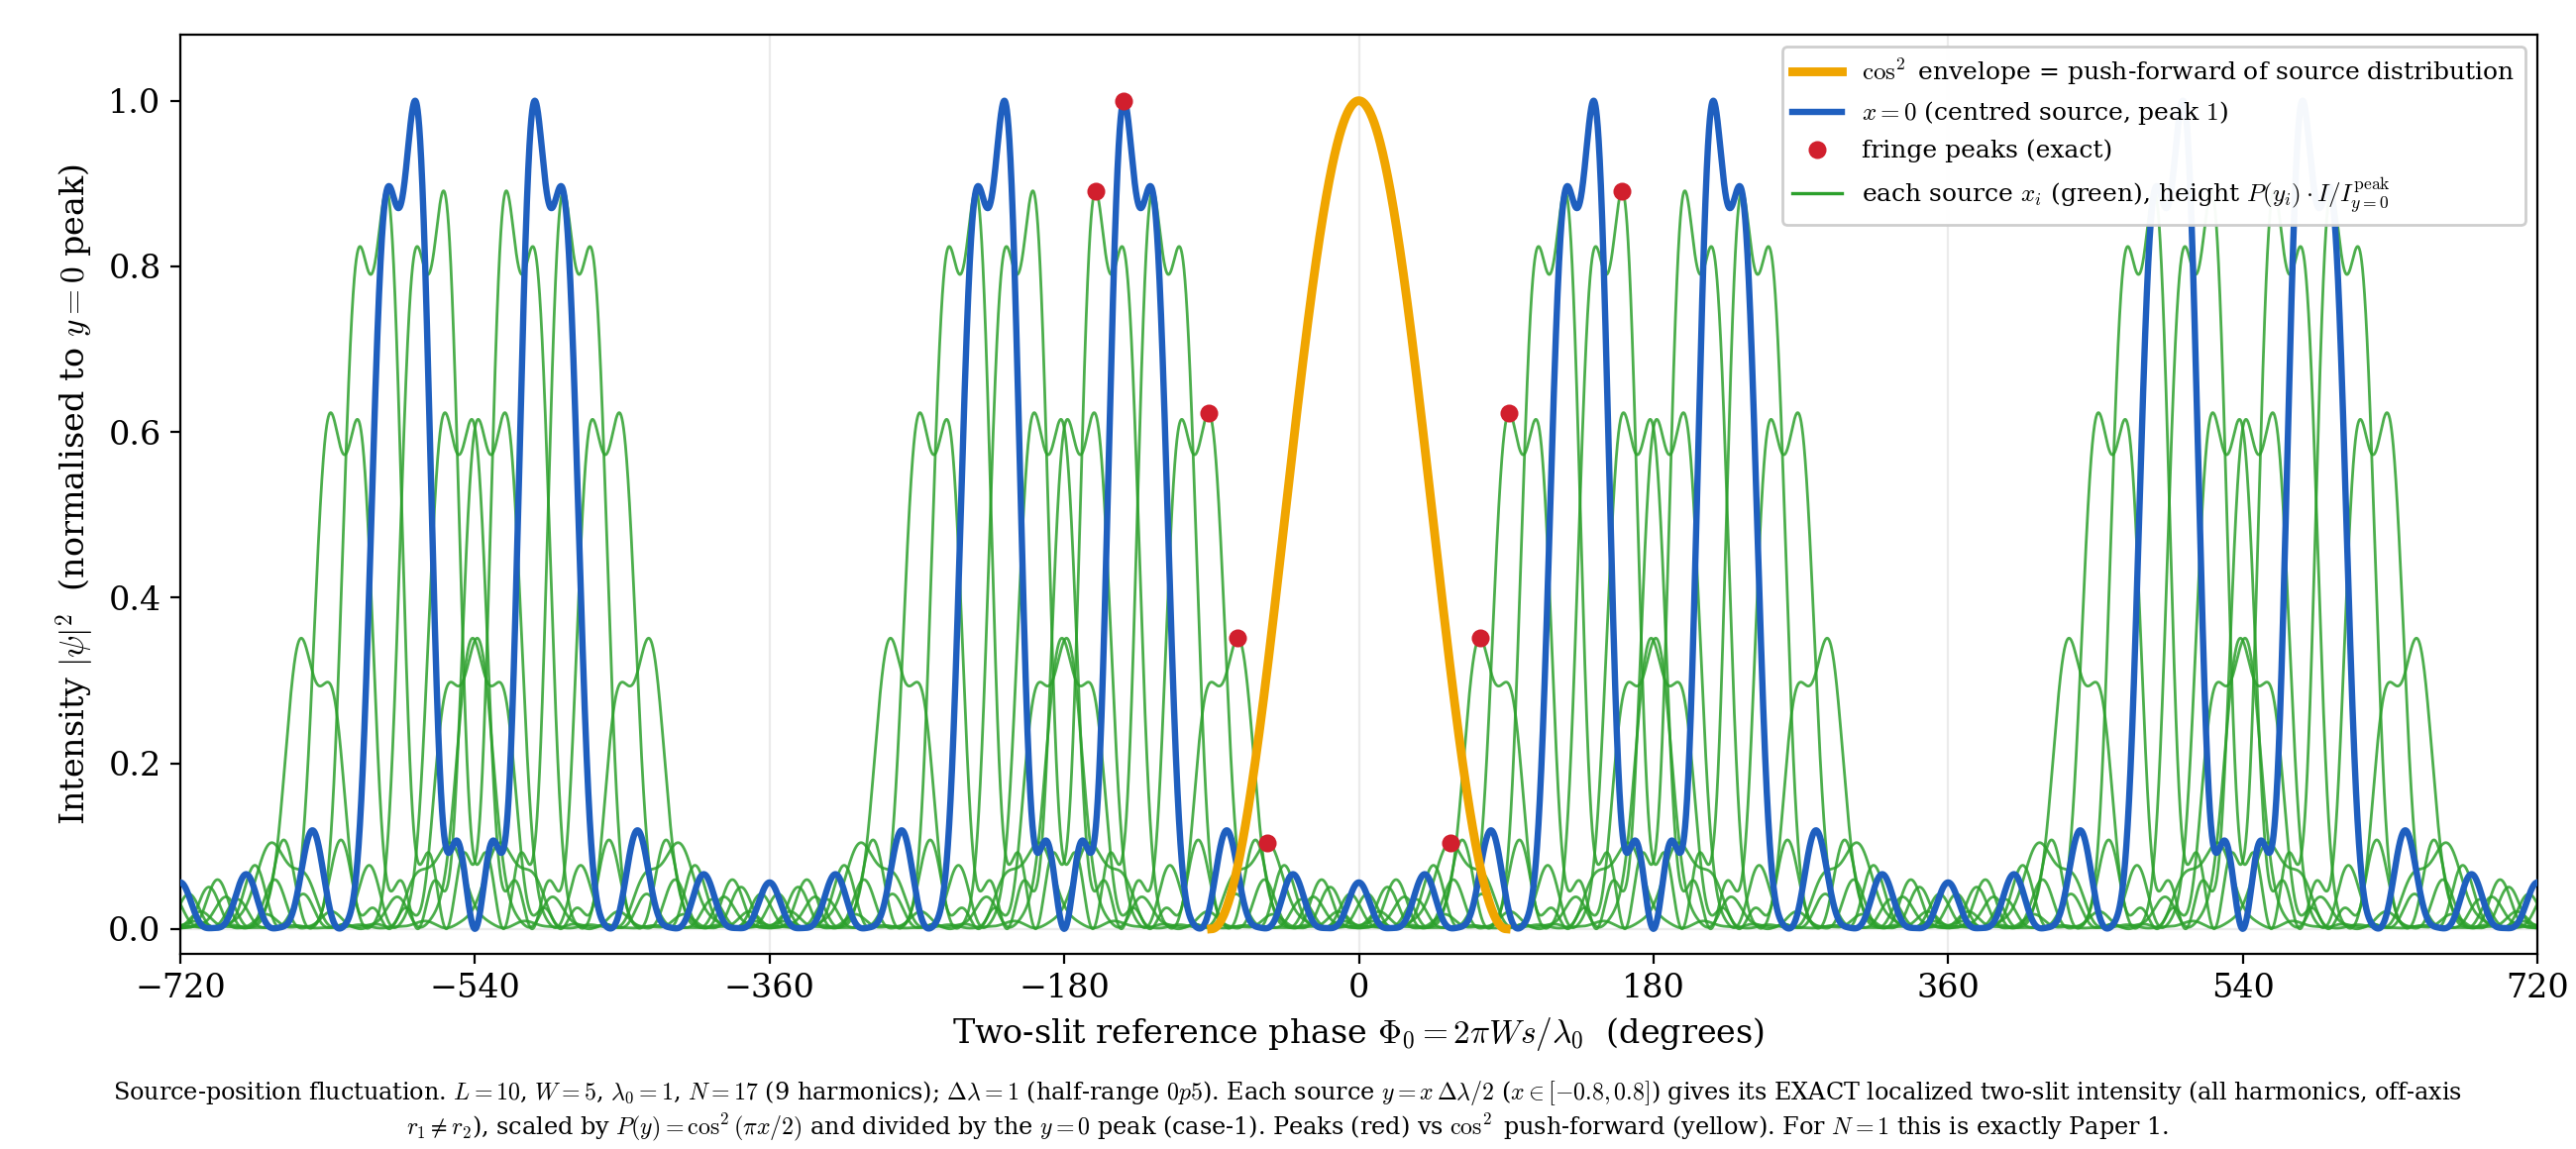
\includegraphics[keepaspectratio,alt={Fig 5 N=17, λ0=1 (misaligned): scattering}]{fig_oddharm_fluct_L10_W5_lam1_N17_dlam1.png}}
\caption{Fig 5 N=17, λ0=1 (misaligned): scattering}
\end{figure}

\emph{Fig 5: \(N=17\), \(\lambda_0=1\) (misaligned,
\(r_k/\lambda_0=10.308\)). Even at \(y=0\) the central peak is only
about \(25\%\) of the ideal \((N+1)^2\), and the fringe peaks of each
source depart greatly from \(\cos^2\) (yellow) --- scattering. Same
geometry and fluctuation as Fig 4, but a mere \(\approx3\%\) difference
in \(\lambda_0\) breaks the interference.}

\textbf{(c) \(N=17\), aligned (\(\lambda_0=1.0308\)).} With
\(\lambda_0\) at the aligned value, \(y=0\) is fully coherent (center
\(=(N+1)^2=324\)). The sharp localized fringe shifts in shape, and the
peaks \textbf{nearly} trace \(\cos^2\) (Fig 6). But off-axis
\(r_1\neq r_2\) breaks the alignment slightly and the peak shifts
\textbf{downward} from \(\cos^2\). This departure splits into two
heterogeneous contributions:

\begin{itemize}
\tightlist
\item
  \textbf{(i) The benign push-forward nonlinearity} (common to all
  \(N\), geometric): from the non-paraxial nature of the map \(u(y)\);
  the departures of \(N=1\) (\(-0.0055\!\sim\!-0.027\)) are this
  (already in {[}1{]}).
\item
  \textbf{(ii) The excess from off-axis scattering} (newly appearing for
  \(N\ge2\)): off-axis \(r_1\neq r_2\) breaks the localization alignment
  and the localized peak itself drops.
\end{itemize}

In the table below, the excess by which the \(N=17\) departure exceeds
\(N=1\) is this new (ii) scattering (strictly, \(N=1\) is
\(\lambda_0=1\) and \(N=17\) is \(\lambda_0=1.0308\), slightly different
geometries so the (i) component is not exactly equal, but the comparison
is broadly valid). For instance at \(x=0.8\) (\(y=0.4\)) the peak is
about \(95\%\) of \(P(y)\) (about \(5\%\) scattering loss), and the
excess grows with \(|y|\).

This off-axis scattering depends on \(W\). The rate of path imbalance at
the center is \(\,\big|dr_1/dy\big|_{y=0}=(W/2)/r_k\propto W\,\), so the
larger \(W\) is, the faster the path leaves the spike (node) when the
source leaves the center, and the more scattering. \textbf{This is the
``true \(W\)-dependence'' foretold in §3.3}, appearing in the off-axis
fragility, not in the central-alignment tolerance band
(\(W\)-independent).

{\def\LTcaptype{none} % do not increment counter
\begin{longtable}[]{@{}
  >{\raggedleft\arraybackslash}p{(\linewidth - 8\tabcolsep) * \real{0.2000}}
  >{\raggedleft\arraybackslash}p{(\linewidth - 8\tabcolsep) * \real{0.2000}}
  >{\raggedleft\arraybackslash}p{(\linewidth - 8\tabcolsep) * \real{0.2000}}
  >{\raggedleft\arraybackslash}p{(\linewidth - 8\tabcolsep) * \real{0.2000}}
  >{\raggedleft\arraybackslash}p{(\linewidth - 8\tabcolsep) * \real{0.2000}}@{}}
\toprule\noalign{}
\begin{minipage}[b]{\linewidth}\raggedleft
\(x\)
\end{minipage} & \begin{minipage}[b]{\linewidth}\raggedleft
peak height
\end{minipage} & \begin{minipage}[b]{\linewidth}\raggedleft
\(\cos^2\) envelope value\(^\dagger\)
\end{minipage} & \begin{minipage}[b]{\linewidth}\raggedleft
departure (\(N=17\) aligned)
\end{minipage} & \begin{minipage}[b]{\linewidth}\raggedleft
ref: departure (\(N=1\))
\end{minipage} \\
\midrule\noalign{}
\endhead
\bottomrule\noalign{}
\endlastfoot
0.2 & 0.9045 & 0.9153 & \(-0.011\) & \(-0.0055\) \\
0.4 & 0.6529 & 0.6899 & \(-0.037\) & \(-0.0178\) \\
0.6 & 0.3404 & 0.4001 & \(-0.060\) & \(-0.0271\) \\
0.8 & 0.0909 & 0.1442 & \(-0.053\) & \(-0.0233\) \\
\end{longtable}
}

\(^\dagger\) The ``\(\cos^2\) envelope value'' is the \textbf{envelope
at the peak position \(p_x\)}, \(\cos^2(\pi p_x/180^\circ)\), not the
weight \(\cos^2(\pi x/2)\) (e.g.~at \(x=0.2\) the envelope value is
\(0.9153\), while the weight \(\cos^2(\pi x/2)=0.9045\)). The
``departure'' in the table is \textbf{peak height \(-\) envelope value}
(envelope basis). The ``about \(95\%\) of \(P(y)\) (scattering loss
\(5\%\))'' in the text is on the \textbf{weight \(P(y)\) basis} and is
the indicator of the pure scattering (ii). The two have different bases.

\begin{figure}
\centering
\pandocbounded{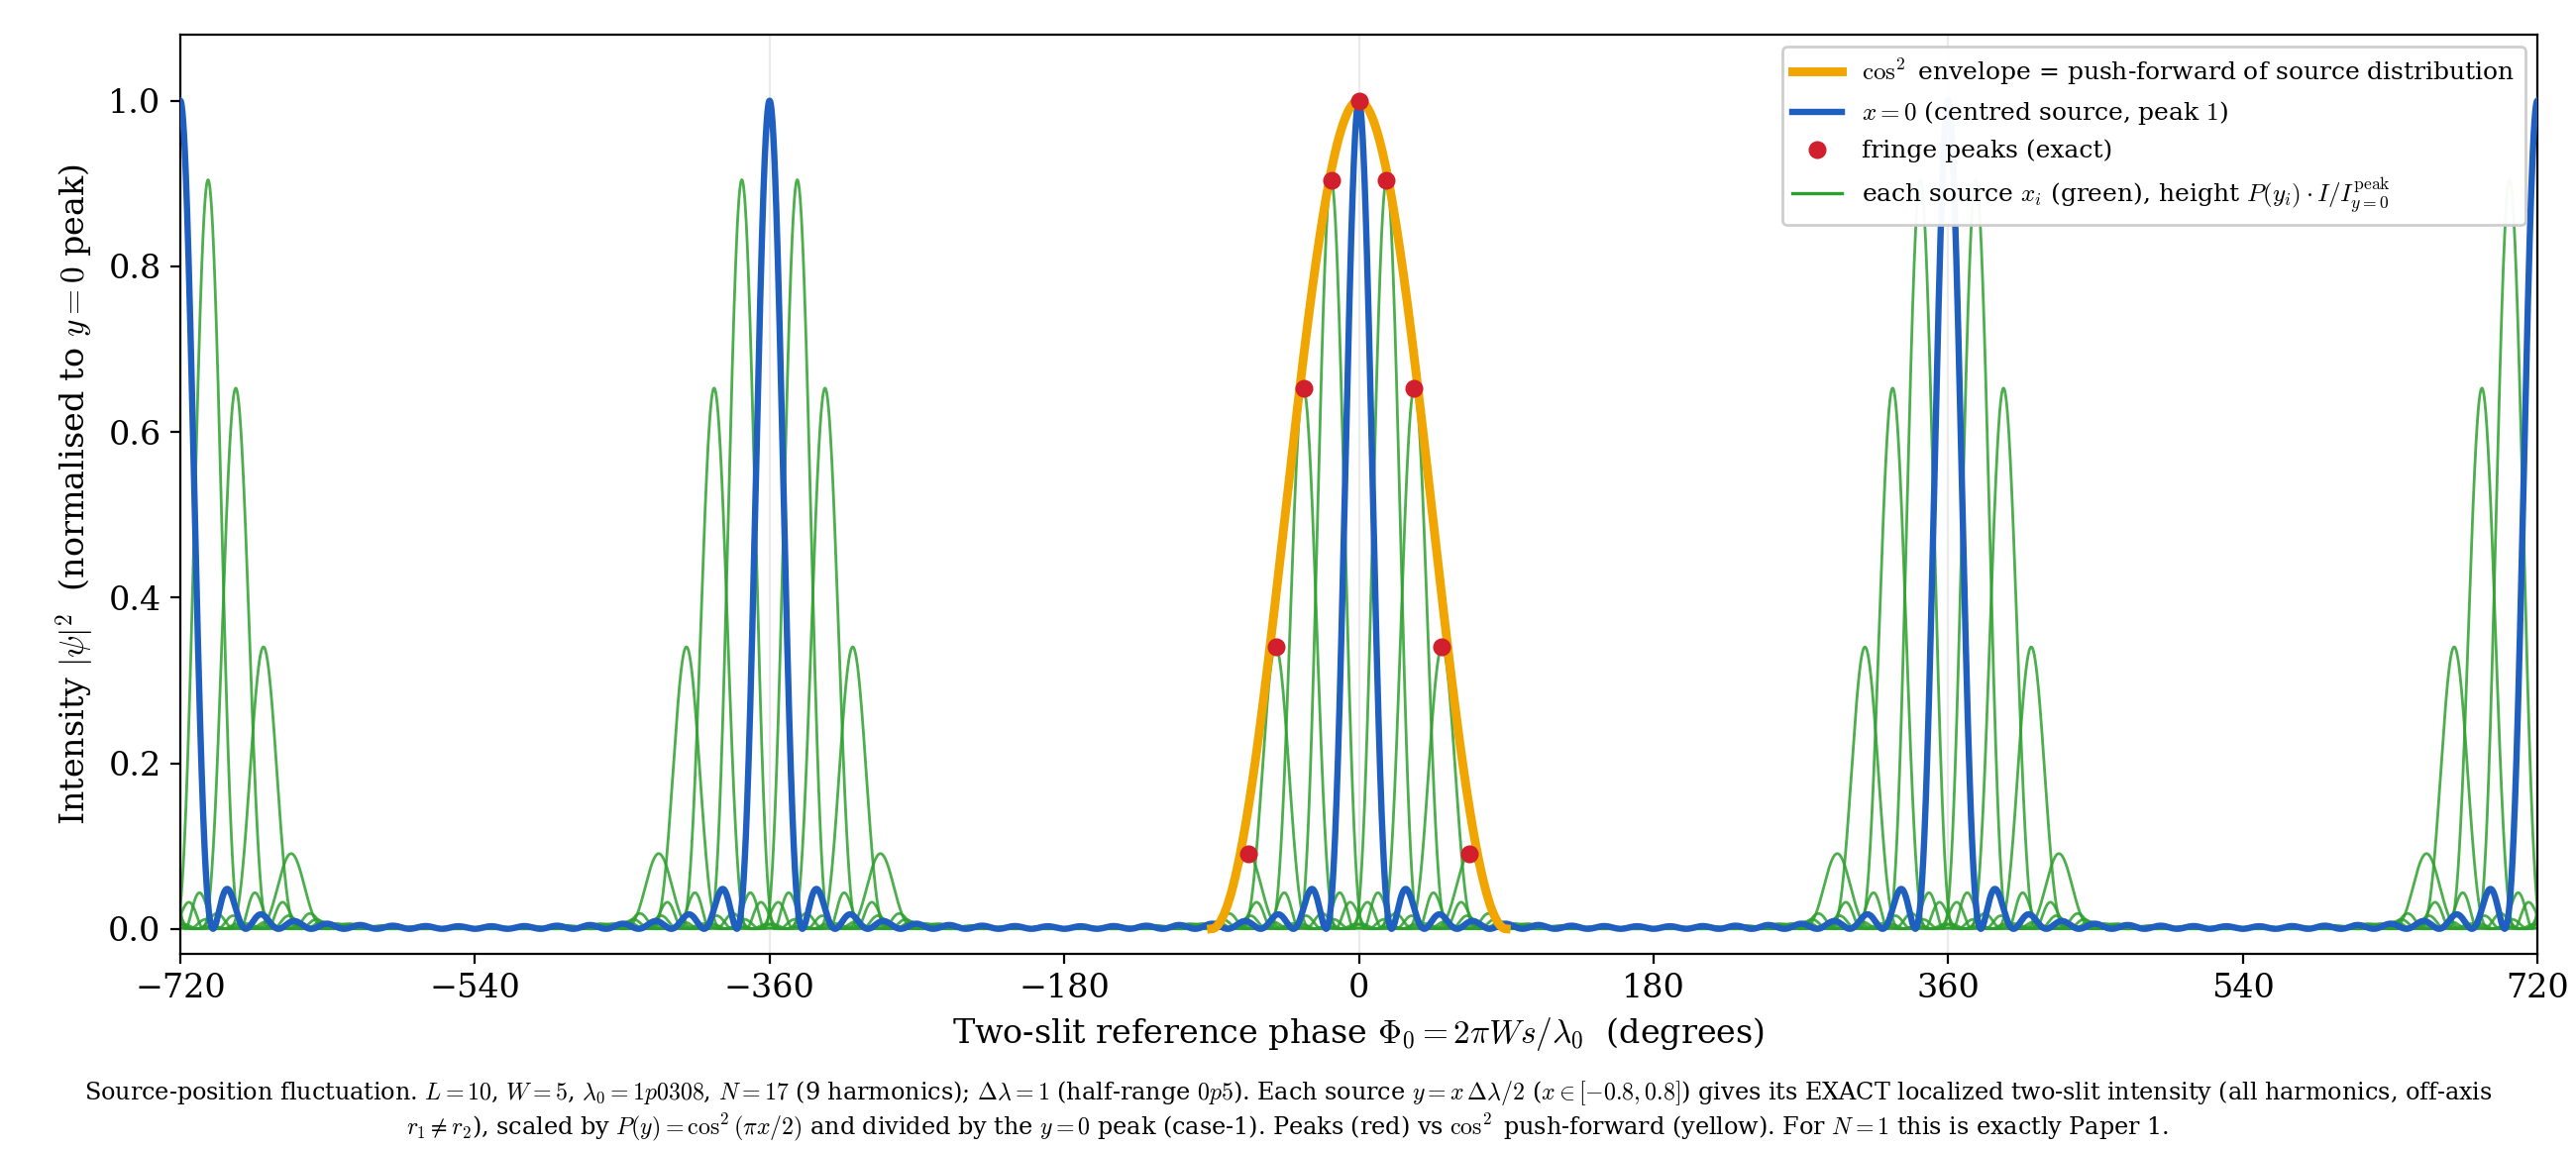
\includegraphics[keepaspectratio,alt={Fig 6 N=17, λ0=1.0308 (aligned): nearly preserves cos²}]{fig_oddharm_fluct_L10_W5_lam1p0308_N17_dlam1.png}}
\caption{Fig 6 N=17, λ0=1.0308 (aligned): nearly preserves cos²}
\end{figure}

\emph{Fig 6: \(N=17\), \(\lambda_0=1.0308\) (aligned,
\(r_k/\lambda_0=10.000\)). At \(y=0\),
\(\mathrm{peak}=323.98\approx18^2\). The sharp localized fringe shifts
along the \(\cos^2\) envelope (yellow), and the peaks (red) nearly trace
\(\cos^2\). Off-axis scattering loss makes the edges shift slightly
below \(\cos^2\) (table above).}

\subsubsection{\texorpdfstring{4.4 \(N\)-dependence of the central
coherence
(\(\lambda_0=1\))}{4.4 N-dependence of the central coherence (\textbackslash lambda\_0=1)}}\label{n-dependence-of-the-central-coherence-lambda_01}

Central coherence at \(y=0\) for \(\lambda_0=1\)
(\(\mathrm{peak}_{y=0}\div\) ideal \((N+1)^2\)):

{\def\LTcaptype{none} % do not increment counter
\begin{longtable}[]{@{}rrrrl@{}}
\toprule\noalign{}
\(N\) & \(\mathrm{peak}_{y=0}\) & ideal \((N+1)^2\) & alignment &
verdict \\
\midrule\noalign{}
\endhead
\bottomrule\noalign{}
\endlastfoot
1 & 4.0 & 4 & \(100\%\) & clean \\
3 & 8.36 & 16 & \(52\%\) & scattered \\
5 & 14.97 & 36 & \(42\%\) & scattered \\
9 & 27.96 & 100 & \(28\%\) & scattered \\
17 & 80.43 & 324 & \(25\%\) & scattered \\
\end{longtable}
}

At \(\lambda_0=1\), only \(N=1\) is aligned; all \(N\ge3\) scatter.
Alignment is decided not by \(N\) itself but by whether
\(r_k/\lambda_0\) falls in the band (3.5).

\begin{center}\rule{0.5\linewidth}{0.5pt}\end{center}

\subsection{\texorpdfstring{5. Verification (\(N=1\) agrees with {[}1{]}
exactly)}{5. Verification (N=1 agrees with {[}1{]} exactly)}}\label{verification-n1-agrees-with-1-exactly}

We directly confirmed that the computational base of this paper agrees
with {[}1{]}. Running our method at \(N=1\) with \(L=10\), \(W=5\),
\(\lambda_0=1\), \(\Delta\lambda=1\) (running the standard program
itself at the same parameters) and comparing with the output of
{[}1{]}'s standard program (fig\_decomposition\_static):

\begin{itemize}
\tightlist
\item
  For all 9 source points the fringe peak position, peak height,
  \(\cos^2\) value, and departure \textbf{agree in every row}.
\item
  Over the whole 16001-point curve, the \textbf{maximum absolute
  difference is \(2.2\times10^{-16}\)} (machine precision).
\item
  The peak value at the center \(y=0\) is \(4.0\) (\(=2^2\), the
  two-slit maximum), confirming that the ``\(y=0\)-peak normalization''
  of this paper is exactly equivalent to the per-fringe normalization of
  {[}1{]} at \(N=1\) (because the two-slit peak is independent of the
  source position \(y\)).
\end{itemize}

Thus \(N=1\) is a special limit of this paper, and {[}1{]} is that case.

\begin{center}\rule{0.5\linewidth}{0.5pt}\end{center}

\subsection{6. Discussion}\label{discussion}

\subsubsection{6.1 Distinction from spatial coherence (van
Cittert--Zernike)}\label{distinction-from-spatial-coherence-van-cittertzernike}

Accumulating the fringes from an extended / multi-point source
\textbf{on an intensity basis} gives a visibility equal to the Fourier
transform of the source brightness distribution: the larger the source,
the fainter the fringes (spatial coherence, van Cittert--Zernike theorem
{[}2,3{]}). This corresponds to observation mode (b) of {[}1{]}
(intensity accumulation \(\to\) visibility loss, not the shape of the
input distribution), an established result.

What this paper (and {[}1{]}) treats is a different mode (a): reading
the fringe \textbf{shift} each trial and histogramming over repetitions
gives the push-forward of the source \textbf{position} distribution,
which \textbf{preserves the shape}. Visibility loss (mode b / vCZ) and
shape preservation (mode a / push-forward) are \textbf{different
observables} and must not be conflated. The novelty here is to extend
this mode (a) to a \textbf{localized odd-harmonic source} and to show
that shape preservation comes with an \textbf{alignment condition (3.4)
and a tolerance band \(\sim1/(2N)\)}, i.e.~a sensitivity to
\(\lambda_0\) --- an aspect absent from vCZ.

\subsubsection{6.2 Scope (and non-claims)}\label{scope-and-non-claims}

What this paper shows is limited to: (i) the alignment condition (3.4)
and its sensitivity (3.5) under which a localized odd-harmonic source
localizes in the double slit while preserving shape; (ii) that an
aligned localized source inherits the \(\cos^2\) readout under
positional fluctuation but the edges shift downward by off-axis
scattering; (iii) that \(N=1\) has none of this fragility and agrees
with {[}1{]} exactly. These are \textbf{illustration and organization}
by exact computation, not the derivation of a new probability law. The
\(\cos^2\) (Born form) that appears is the push-forward of the input
\(P(y)=\cos^2\); we do not ask the origin of the probability
interpretation, the squaring rule, or randomness. We do not claim
``derivation of the Born rule'' or ``solution of the measurement
problem.''

\subsubsection{6.3 Implications of the sensitivity (limited
remark)}\label{implications-of-the-sensitivity-limited-remark}

That a slight difference in \(\lambda_0\) (\(\sim 1/(2N)\)) decides
interference vs scattering, that the required precision tightens as
\(N\) (the sharpness of localization) grows, and that the larger \(W/L\)
the greater the off-axis (under-fluctuation) fragility (\textbf{while
the central-alignment tolerance band itself is independent of \(W/L\)}),
are consequences of exact computation for our configuration. Between
resolution (sharpness of localization \(\propto N\)) and robustness
(alignment / fluctuation tolerance) there is a trade-off controlled by
\(N\). We give no physical interpretation beyond this observation.

\begin{center}\rule{0.5\linewidth}{0.5pt}\end{center}

\subsection{7. Conclusion}\label{conclusion}

For far-field double-slit interference from a \textbf{localized
odd-harmonic source} with positional fluctuation, exact computation on
the same geometry as {[}1{]} shows the following.

\begin{enumerate}
\def\labelenumi{\arabic{enumi}.}
\tightlist
\item
  Representing the localization by the odd-harmonic sum \(S_N\), the far
  field gives a single, sharply localized fringe at the center while
  preserving shape. But this requires the alignment condition
  \(\sqrt{L^2+(W/2)^2}=(m/2)\lambda_0\) that the diagonal distance be an
  integer/half-integer multiple of the fundamental wavelength.
\item
  Alignment is a band of width \(\sim1/(2N)\), narrower as \(N\) (the
  sharpness of localization) grows. A \(\approx3\%\) difference in
  \(\lambda_0\) separates interference from scattering. The
  central-alignment tolerance band itself is independent of \(W/L\), but
  the larger \(W/L\) the greater the off-axis (under-fluctuation)
  fragility.
\item
  An aligned localized source still traces \(\cos^2\) in the
  fringe-shift distribution under positional fluctuation (inheriting the
  push-forward of {[}1{]}), but off-axis scattering shifts the edges
  downward from \(\cos^2\). The single wavelength \(N=1\) has none of
  this fragility and is unconditional; running this paper at \(N=1\)
  under the same conditions agrees with {[}1{]} to machine precision.
\end{enumerate}

In short, the net finding of this paper is that \textbf{localization
(\(N\ge2\)) does not improve the push-forward of {[}1{]}; it adds an
alignment constraint and off-axis fragility} --- i.e.~\textbf{shape
preservation is conditional and fragile, and \(N=1\) is the robust
special case.} This is a negative result --- that localization
complicates and weakens the readout --- rather than a positive ``shape
preservation,'' and for the program from localized waves toward Born
statistics this fragility is the important implication.

This is not the derivation of a new probability law but an extension of
the input-distribution push-forward ({[}1{]}) to a localized source,
illustrating and organizing the alignment condition / sensitivity /
fluctuation tolerance (and its fragility) of the interference. It is a
different observation mode from the visibility loss of an extended
source (spatial coherence / vCZ {[}2,3{]}). This paper is a thought
experiment; it organizes established physics rather than overturning it.

\begin{center}\rule{0.5\linewidth}{0.5pt}\end{center}

\subsection{References}\label{references}

{[}1{]} Noriaki Kihara, ``A Thought Experiment on Double-Slit
Interference from a Source with Positional Fluctuation --- Push-forward
of the Source-Position Distribution to the Fringe-Shift Distribution
(Shape Preservation),'' Zenodo, v0.3 (2026), Concept DOI:
10.5281/zenodo.21035808 / Version DOI: 10.5281/zenodo.21035809 (the
starting point and sole self-reference).

{[}2{]} M. Born and E. Wolf, \emph{Principles of Optics}, 7th (expanded)
ed.~(Cambridge University Press, 1999) (far-field double slit, partial
coherence, van Cittert--Zernike theorem).

{[}3{]} L. Mandel and E. Wolf, \emph{Optical Coherence and Quantum
Optics} (Cambridge University Press, 1995) (spatial coherence and the
van Cittert--Zernike theorem).

{[}4{]} T. Takagi, \emph{Kaiseki Gairon} (Introduction to Analysis), 3rd
rev. ed.~(Iwanami Shoten, 1961) (trigonometric series, the closed form
of the cosine sum of an arithmetic progression, the Dirichlet kernel).

\begin{center}\rule{0.5\linewidth}{0.5pt}\end{center}

\subsection{Appendix: Reproduction
code}\label{appendix-reproduction-code}

All results are reproduced by the following exact-computation scripts
(all angles and paths derived from \(L,W,\lambda_0\); no constants
placed arbitrarily; no motion assumption or Doppler).

\begin{itemize}
\tightlist
\item
  Interference / fluctuation engine:
  \texttt{fig\_oddharm\_interference.py}

  \begin{itemize}
  \tightlist
  \item
    Aligned shape-preserving interference (Fig 2):
    \texttt{-\/-L\ 10\ -\/-W\ 5\ -\/-lam0\ 1.0308\ -\/-N\ 17\ -\/-halfdeg\ 180}
  \item
    Positional-fluctuation readout (Figs 4--6): add \texttt{-\/-dlam\ 1}
    with \texttt{-\/-N\ 1} (\(\lambda_0=1\)) / \texttt{-\/-N\ 17}
    (\(\lambda_0=1\)) / \texttt{-\/-N\ 17\ -\/-lam0\ 1.0308}
  \end{itemize}
\item
  Localized source wave \(S_N\) (Fig 1):
  \texttt{make\_paper2\_localized\_wave.py}
\item
  Standard program of {[}1{]} (basis of the verification; the setup of
  Fig 3): \texttt{fig\_decomposition\_static.py},
  \texttt{fig\_setup\_source\_uncertainty.py}
\end{itemize}

The fluctuation mode computes (3.2) exactly at each source
\(y=x\,\Delta\lambda/2\) (\(x\in[-0.8,0.8]\)) over all harmonics,
off-axis (\(r_1\neq r_2\)), with the source-side phase, weights by
\(P(y)=\cos^2(\pi x/2)\), and normalizes by the central peak at \(y=0\)
(case-1 normalization). At \(N=1\) this agrees with {[}1{]} to machine
precision (§5).

\end{document}
